\documentclass[12pt]{article}
% Full article preamble (duplicated, no common file)
\usepackage{fontspec}
\usepackage[a4paper,margin=2.5cm,includefoot]{geometry}
\usepackage{polyglossia}
\usepackage{amsmath}
\usepackage{amssymb}
\usepackage{xcolor}
\usepackage{fancyhdr}
\usepackage{graphicx}
\usepackage{listings}
\usepackage[most]{tcolorbox}
\usepackage{pifont}
\usepackage{enumitem}
\usepackage{titlesec}
\usepackage[bottom]{footmisc}
\usepackage{titling}
\usepackage{minted}
\usepackage{etoolbox}
\usepackage{array}
\usepackage{extsizes}

\newfontfamily\emoji{Segoe UI Emoji}

\pagestyle{fancy}

\setmainlanguage[numerals=western]{arabic}
\setotherlanguage{english}
\newfontfamily\arabicfont[Script=Arabic]{Amiri}
\newfontfamily\arabicfonttt[Script=Arabic]{Courier New}

\lstset{
  language=[Sharp]C,
  numbers=left,
  stepnumber=1,
  numbersep=8pt,
  frame=single,
  basicstyle=\ttfamily\small,
  keywordstyle=\color{blue},
  stringstyle=\color{red},
  commentstyle=\color{green!50!black}
}

\newif\ifdetailed
\ifdefined\setdetailed
  \setdetailed
\fi

\newif\ifwithsols
\ifdefined\setwithsols
  \setwithsols
\fi

% unified tcolorboxes for articles
\tcbset{colback=white, colframe=black, fonttitle=\bfseries, boxrule=0.8pt}
\newtcolorbox{boxDef}[1][]{colback=blue!5!white,colframe=blue!75!black,
  title={{\emoji📘} تعريف\ifx\\#1\\\else ~#1\fi :}}
\newtcolorbox{boxExercise}[1][]{colback=cyan!5!white,colframe=cyan!70!black,
  title={{\emoji🧩} تمرين\ifx\\#1\\\else ~#1\fi :}}
\newtcolorbox{boxExample}[1][]{colback=yellow!5!white,colframe=orange!90!black,
  title={{\emoji📝} مثال\ifx\\#1\\\else ~#1\fi :}}
\newtcolorbox{boxNote}[1][]{colback=gray!10!white,colframe=black,
  title={{\emoji✨} ملاحظة\ifx\\#1\\\else ~#1\fi :}}
\newtcolorbox{boxAttention}[1][]{colback=magenta!10!white,colframe=magenta!80!black,
  title={{\emoji🔔} تنبيه\ifx\\#1\\\else ~#1\fi :}}
\newtcolorbox{boxWarning}[1][]{colback=red!5!white,colframe=red!75!black,
  title={{\emoji⚡} ملاحظة هامة\ifx\\#1\\\else ~#1\fi :}}
\newtcolorbox{boxSolution}[1][]{colback=green!5!white,colframe=green!60!black,
  title={{\emoji✅} حل\ifx\\#1\\\else ~#1\fi :}}
\newtcolorbox{boxSymbol}[1][]{colback=purple!5!white,colframe=purple!70!black,
  title={{\emoji🔣} رمز\ifx\\#1\\\else ~#1\fi :}}

\tcbset{simplecode/.style={ colback=gray!5, colframe=black!50, boxrule=0.4pt, arc=2pt, left=4pt,right=4pt,top=4pt,bottom=4pt}}
\newenvironment{boxCode}{\begin{tcolorbox}[simplecode]}{\end{tcolorbox}}

\newcolumntype{C}[1]{>{\centering\arraybackslash}p{#1}}

% redefine spaces after titles
\makeatletter
\renewcommand{\@maketitle}{%
  \begin{center}
    {\huge \bfseries \@title \par}%
    \vskip 0.2em % space between title and author
    {\large \@author \par}%
    % \vskip 0.2em % space between author and date
    % {\normalsize \@date \par}%
  \end{center}
}
\makeatother

\fancyhf{} % clear default
\fancypagestyle{plain}{
  \fancyhf{}
  \fancyhead[L]{مدرسة التسامح الشاملة}
  % \fancyhead[L]{
\includegraphics[height=1cm]{../../../images/logoTasamoh.png}}
  \fancyhead[R]{الأستاذ محمود اغبارية}
  \fancyfoot[C]{\thepage}
}

\fancyhead[L]{مدرسة التسامح الشاملة}
\fancyhead[R]{الأستاذ محمود اغبارية}
\fancyfoot[C]{\thepage}
% \date{\today}

\setcounter{tocdepth}{3} % only section subsection and subsubsection in TOC


% ----------------------


% \begin{document}

% \maketitle

% % \clearpage  % start TOC on a new page
% % \renewcommand{\contentsname}{جدول المحتويات}
% % \tableofcontents
% % \clearpage

% \part*{part 1} % the * prevents numbering
% \section*{مقدمة}
% \subsection*{مثال رياضي}
% \subsubsection*{مثال فرعي}
% \paragraph*{ paragraph 1}
% \subparagraph*{sub paragraph 1}

% \ifdetailed
% \begin{english}
% \begin{minted}{csharp}
% // C# Example
% \end{minted}
% \end{english}
% \fi

% OLD WAY
% \ifdetailed
% \begin{english}
% \begin{lstlisting}
% // C# Example
% \end{lstlisting}
% \end{english}
% \fi

% % 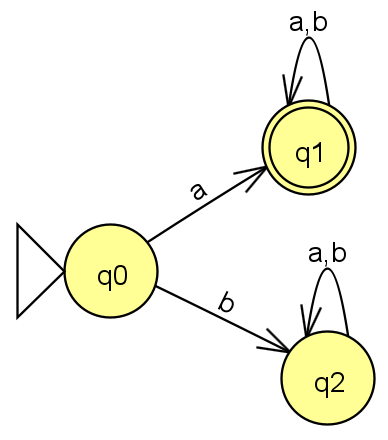
\includegraphics[width=0.2\textwidth]{../../../images/DFAs/ex1_q1.png}



% \vspace{3cm}
% \begin{flushleft}
% أرجو لكم وقتًا ممتعًا.

% الأستاذ محمود اغبارية.
% \end{flushleft}


% \end{document}


\title{تمارين للاختيار للامتحان}

\begin{document}
\maketitle
\thispagestyle{fancy}

\begin{enumerate}[itemsep=2em]
\item
اكتب برنامجًا يستقبل عددين صحيحين، على البرنامج أن يعيد حاصل طرح العدد الصغير من العدد الكبير.

\ifwithsols
\begin{boxSolution}
\begin{english}
\begin{minted}{csharp}
int a = int.Parse(Console.ReadLine());
int b = int.Parse(Console.ReadLine());
Console.WriteLine(Math.Abs(a - b));
\end{minted}
\end{english}
الفكرة: استخدام \textenglish{Math.Abs} لاستخراج الفرق المطلق.
\end{boxSolution}
\fi


\item
اكتب برنامجًا يستقبل عددين ويطبع \textenglish{"Consecutive"} إذا كانا متتاليين، و \textenglish{"Not Consecutive"} إذا لم يكونا متتاليين.

\ifwithsols
\begin{boxSolution}
\begin{english}
\begin{minted}{csharp}
int a = int.Parse(Console.ReadLine());
int b = int.Parse(Console.ReadLine());
if (Math.Abs(a - b) == 1)
    Console.WriteLine("Consecutive");
else
    Console.WriteLine("Not Consecutive");
\end{minted}
\end{english}
\end{boxSolution}
\fi


\item
اكتب برنامجًا يتلقى عددين صحيحين وموجبين، العدد الأول مؤلف من منزلتين والعدد الثاني مؤلف من منزلة واحدة، على البرنامج أن يطبع \textenglish{Yes} إذا كان العدد الثاني هو إحدى منازل العدد الأول.

\ifwithsols
\begin{boxSolution}
\begin{english}
\begin{minted}{csharp}
int n = int.Parse(Console.ReadLine());  // two digits
int d = int.Parse(Console.ReadLine());  // one digit
int tens = n / 10;
int ones = n % 10;
if (d == tens || d == ones)
    Console.WriteLine("Yes");
else
    Console.WriteLine("No");
\end{minted}
\end{english}
\end{boxSolution}
\fi


\item
اكتب برنامجًا يستقبل عددًا صحيحا موجبًا، على البرنامج أن يطبع الرّقم الزوجي التالي لهذا الرقم.\\
مثال: إذا استقبل العدد 5، على البرنامج أن يطبع 6. وإذا استقبل 6 على البرنامج أن يطبع 8.

\ifwithsols
\begin{boxSolution}
\begin{english}
\begin{minted}{csharp}
int x = int.Parse(Console.ReadLine());
int nextEven;
if (x % 2 == 0)
    nextEven = x + 2;
else
    nextEven = x + 1;
Console.WriteLine(nextEven);
\end{minted}
\end{english}
\end{boxSolution}
\fi


\item
اكتب برنامجًا يستقبل ثلاثة أعداد صحيحة، إذا كانت كل الأعداد زوجية فعلى البرنامج أن يطبع معدّلها، خلاف ذلك يطبع حاصل جمعها.

\ifwithsols
\begin{boxSolution}
\begin{english}
\begin{minted}{csharp}
int a = int.Parse(Console.ReadLine());
int b = int.Parse(Console.ReadLine());
int c = int.Parse(Console.ReadLine());
if (a % 2 == 0 && b % 2 == 0 && c % 2 == 0)
{
    double avg = (a + b + c) / 3.0;
    Console.WriteLine(avg);
}
else
{
    Console.WriteLine(a + b + c);
}
\end{minted}
\end{english}
\end{boxSolution}
\fi


\item
اكتب برنامجًا يستقبل عددًا ويحذف المنزلة الثالثة (منزلة المئات) من العدد.\\
مثال: إذا استقبل العدد 6543، على البرنامج أن يطبع 643. وإذا استقبل العدد 745636، على البرنامج أن يطبع 74536.

\ifwithsols
\begin{boxSolution}
الفكرة: قسمة على 1000 لاستخراج الجزء الأيسر، وأخذ \textenglish{mod 100} لاستخراج الآحاد والعشرات، ثم تجميعهما.
\begin{english}
\begin{minted}{csharp}
int n = int.Parse(Console.ReadLine());
int left = n / 1000;
int right = n % 100;
int result = left * 100 + right;
Console.WriteLine(result);
\end{minted}
\end{english}
\end{boxSolution}
\fi


\item
تتبع مقطع الكود التالي ثم املأ الجدول الذي بعده:

\begin{boxCode}
\begin{english}
\begin{minted}{csharp}
int n = int.Parse(Console.ReadLine());
int a = n / 1000;
int b = n % 100;
int result = a * 100 + b;
Console.WriteLine(result);
\end{minted}
\end{english}
\end{boxCode}



\begin{enumerate}
    \item
    \textbf{املأ الجدول التالي:} لكل واحدة من قيم $n$، اكتب ماذا تكون قيمة $a, b$ وما هي القيمة التي يطبعها البرنامج:
\begin{center}
% \begin{tabular}{|c|c|c|c|c|}

\begin{tabular}{|C{2cm}|C{3cm}|C{3cm}|C{3cm}|C{3cm}|}
\hline
\large{\textbf{$n$}} & \large{\textbf{$a$}} & \large{\textbf{$b$}} & \large{\textenglish{\textbf{result}}} \\
\hline
7654 &  &  &  \\
\hline
32154 &  &  &  \\
\hline
8111 &  &  &  \\
\hline
354 &  &  &  \\
\hline
1 &  &  &  \\
\hline
\end{tabular}
\end{center}

\item
أعط قيمة لـ $n$ تجعل البرنامج يطبع $111$.

\item
ما هي وظيفة البرنامج أعلاه؟ (بسطر واحد)
\end{enumerate}


\item
اكتب برنامجًا يستقبل عددًا مكوّنًا من 6 منازل، على البرنامج أن يكوّن رقمًا جديدًا من 3 منازل بحيث يأخذ من العدد الأصلي منزلة الآحاد والمئات وعشرات الآلاف.\\
مثال: إذا استقبل العدد 765325، على البرنامج أن يطبع 635.

\ifwithsols
\begin{boxSolution}
\begin{english}
\begin{minted}{csharp}
int n = int.Parse(Console.ReadLine()); // abcdef (a=hundred-thousands)
int ones = n % 10;                 // f
int hundreds = (n / 100) % 10;     // d
int tenThousands = (n / 10000) % 10; // b
int result = tenThousands * 100 + hundreds * 10 + ones; // b d f
Console.WriteLine(result);
\end{minted}
\end{english}
\end{boxSolution}
\fi


\item
في مثلث متساوي الأضلاع، كل الأضلاع لها نفس الطول.\\
إذا كان طول ضلع مثلث متساوي الأضلاع هو $a$. فإنّ: \\
ارتفاع المثلث $a \times \frac{\sqrt{3}}{2} =$\\
مساحة المثلث $a^2 \times \frac{\sqrt{3}}{4} =$\\
اكتب برنامجًا يستقبل طول ضلع مثلث متساوي الأضلاع.
على البرنامج أن يطبع ارتفاع المثلث ومساحته.

\ifwithsols
\begin{boxSolution}
\begin{english}
\begin{minted}{csharp}
double s = double.Parse(Console.ReadLine());
double h = s * Math.Sqrt(3) / 2.0;
double area = Math.Pow(s, 2) * Math.Sqrt(3) / 4.0;
Console.WriteLine($"Height = {h}");
Console.WriteLine($"Area = {area}");
\end{minted}
\end{english}
\end{boxSolution}
\fi


\item
لكل نقطتين $(x_1,y_1)$ و $(x_2,y_2)$، في المستوى، يمكن حساب ميل الخط المستقيم الذي يمرّ بينهما باستخدام المعادلة التالية:
\[ m = \frac{y_2 - y_1}{x_2 - x_1} \]
اكتب برنامجًا يستقبل إحداثيات نقطتين في المستوى، ويطبع:
\begin{itemize}
\item    \textenglish{Infinity} إذا كان \(x_2 - x_1 = 0\). \\
\item    وفي باقي الحالات يطبع الميل.
\end{itemize}

\ifwithsols
\begin{boxSolution}
تنبيه: عندما يكون \(x_2 - x_1 = 0\) يكون الميل غير معرّف.
\begin{english}
\begin{minted}{csharp}
double x1 = double.Parse(Console.ReadLine());
double y1 = double.Parse(Console.ReadLine());
double x2 = double.Parse(Console.ReadLine());
double y2 = double.Parse(Console.ReadLine());
double dx = x2 - x1;
if (dx == 0)
    Console.WriteLine("Infinity");
else
    Console.WriteLine((y2 - y1) / dx);
\end{minted}
\end{english}
\end{boxSolution}
\fi


\item
كل مثلث في المستوى يجب أن يحقق قانون بناء المثلث وهو أنّ مجموع كل ضلعين أكبر من الثالث. \\
 أي إذا كانت أضلاعه $a, b, c$ فإنّه يجب أن يحقق الشروط التالية:
\begin{align*}
a + b &> c \\
a + c &> b \\
b + c &> a
\end{align*}

اكتب برنامجًا يستقبل ثلاثة أطوال، على البرنامج أن يفحص إذا كانت هذه الأرقام تحقق قانون بناء المثلث أم لا. \\
إذا كانت تحقق قانون بناء المثلث فعلى البرنامج أن يطبع \textenglish{"Legal"}.
وإلا فإنّه يطبع \textenglish{"Not Legal"}.

مثال: الأطوال $3, 4, 5$ تحقق قانون بناء المثلث، لأنّ $3 + 4 > 5$ و $3 + 5 > 4$ و $4 + 5 > 3$. ففي هذه الحالة على البرنامج أن يطبع \textenglish{"Legal"}. \\
أمّا الأطوال $3, 4, 9$ لا تحقق قانون بناء المثلث، لأنّ $3 + 4 < 9$، ففي هذه الحالة على البرنامج أن يطبع \textenglish{"Not Legal"}.


\ifwithsols
\begin{boxSolution}
\begin{english}
\begin{minted}{csharp}
int a = int.Parse(Console.ReadLine());
int b = int.Parse(Console.ReadLine());
int c = int.Parse(Console.ReadLine());
bool ok = a + b > c && a + c > b && b + c > a;
if (ok)
    Console.WriteLine("Legal");
else
    Console.WriteLine("Not Legal");
\end{minted}
\end{english}
\end{boxSolution}
\fi

\clearpage
\item
تتبع الكود التالي ثم املأ الجدول الذي بعده.

\begin{boxCode}
\begin{english}
\begin{minted}{csharp}
int x = int.Parse(Console.ReadLine());
int y = int.Parse(Console.ReadLine());

if (Math.Abs(x - y) < 3)
    Console.WriteLine("Close");
else if (x > y)
    Console.WriteLine("First");
else
    Console.WriteLine("Second");
\end{minted}
\end{english}
\end{boxCode}

\textbf{املأ الجدول التالي:}
\begin{center}
\begin{tabular}{|c|c|c|c|c|}
\hline
\textbf{x} & \textbf{y} & \textenglish{Math.Abs(x - y) < 3} & \textenglish{x > y} & \textbf{Output} \\
\hline
4 & 2 & True & True & Close \\
\hline
5 & 6 &  &  &  \\
\hline
10 & 6 &  &  &  \\
\hline
3 & 8 &  &  &  \\
\hline
 &  &  &  & First \\
\hline
 &  &  &  & Second \\
\hline
\end{tabular}
\end{center}

\ifwithsols
\begin{boxSolution}
المخرج: \textenglish{Close} لأن الفرق المطلق يساوي 2 وهو أصغر من 3.\\
مثال آخر يعطي نفس المخرج: \textenglish{7} و\textenglish{6}.
\end{boxSolution}
\fi


\item
تتبع الكود التالي ثم املأ الجدول الذي بعده.

\begin{boxCode}
\begin{english}
\begin{minted}{csharp}
int a = int.Parse(Console.ReadLine());
int b = int.Parse(Console.ReadLine());
int c = int.Parse(Console.ReadLine());

int diff = Math.Abs(Math.Max(a, b) - c);
Console.WriteLine(diff);
\end{minted}
\end{english}
\end{boxCode}

\textbf{املأ الجدول التالي:}

\begin{center}
\begin{tabular}{|c|c|c|c|}
\hline
\textbf{a} & \textbf{b} & \textbf{c} & \textbf{diff/output} \\
\hline
5 & 2 & 7 & 2 \\
\hline
3 & 9 & 4 &  \\
\hline
10 & 10 & 6 &  \\
\hline
1 & 8 & 9 &  \\
\hline
 &  &  & 0 \\
\hline
 &  &  & 5 \\
\hline
\end{tabular}
\end{center}

\ifwithsols
\begin{boxSolution}
\textenglish{Max(5,2) = 5} ثم \(\lvert 5 - 7 \rvert = 2\) لذا المخرج \textenglish{2}.
\end{boxSolution}
\fi

\clearpage
\item
تتبع الكود التالي ثم املأ الجدول الذي بعده.

\begin{boxCode}
\begin{english}
\begin{minted}{csharp}
int x = int.Parse(Console.ReadLine());

if (x % 2 == 0 && x % 4 == 0)
    Console.WriteLine("Double Even");
else if (x % 2 == 0)
    Console.WriteLine("Even");
else
    Console.WriteLine("Odd");
\end{minted}
\end{english}
\end{boxCode}

\textbf{املأ الجدول التالي:}
\begin{center}
\begin{tabular}{|c|c|c|c|}
\hline
\textbf{x} & \textenglish{x \% 2 == 0} & \textenglish{x \% 4 == 0} & \textbf{Output} \\
\hline
8 & True & True & Double Even \\
\hline
6 &  &  &  \\
\hline
9 &  &  &  \\
\hline
4 &  &  &  \\
\hline
 &  &  & Double Even \\
\hline
 &  &  & Odd \\
\hline
\end{tabular}
\end{center}

\ifwithsols
\begin{boxSolution}
عند \textenglish{x = 8}: القسمة على 2 وعلى 4 بدون باقٍ، إذًا المخرج \textenglish{Double Even}.\\
مثال آخر: \textenglish{12} أيضًا يعطي \textenglish{Double Even}.
\end{boxSolution}
\fi

\item
تتبع الكود التالي ثم املأ الجدول الذي بعده.

\begin{boxCode}
\begin{english}
\begin{minted}{csharp}
int a = int.Parse(Console.ReadLine());
int b = int.Parse(Console.ReadLine());
int c = int.Parse(Console.ReadLine());

if (a > b && b > c)
    Console.WriteLine("Descending");
else if (a < b && b < c)
    Console.WriteLine("Ascending");
else
    Console.WriteLine("Mixed");
\end{minted}
\end{english}
\end{boxCode}

\textbf{املأ الجدول التالي:}

\begin{center}
\begin{tabular}{|c|c|c|c|c|c|}
\hline
\textbf{a} & \textbf{b} & \textbf{c} & \textenglish{a > b \&\& b > c} & \textenglish{a < b \&\& b < c} & \textbf{Output} \\
\hline
3 & 7 & 5 & False & False & Mixed \\
\hline
9 & 7 & 1 &  &  &  \\
\hline
2 & 3 & 4 &  &  &  \\
\hline
5 & 5 & 6 &  &  &  \\
\hline
 &  &  &  &  & Ascending \\
\hline
 &  &  &  &  & Descending \\
\hline
\end{tabular}
\end{center}

\ifwithsols
\begin{boxSolution}
\textenglish{3 < 7} لكن \textenglish{7 > 5}، ليست تصاعدية ولا تنازلية، إذًا \textenglish{Mixed}.
\end{boxSolution}
\fi


\item
تتبع الكود التالي ثم املأ الجدول الذي بعده.
\begin{boxCode}
\begin{english}
\begin{minted}{csharp}
int age;
bool hasTicket;

if (age > 10 && hasTicket || age == 5)
{
    Console.WriteLine("Allowed");
}
else
{
    Console.WriteLine("Not Allowed");
}
\end{minted}
\end{english}
\end{boxCode}


\textbf{املأ الجدول التالي:}

\begin{center}
\begin{tabular}{|c|c|c|c|}
\hline
\textbf{age} & \textbf{hasTicket} & \textenglish{age > 10 \&\& hasTicket || age == 5} & \textbf{Output} \\
\hline
12 & True & True & Allowed \\
\hline
12 & False &  &  \\
\hline
5 & False &  &  \\
\hline
9 & True &  &  \\
\hline
 &  &  & Allowed \\
\hline
 &  &  & Not Allowed \\
\hline
\end{tabular}
\end{center}


\ifwithsols
\begin{boxSolution}
حسب أسبقية العمليات: \(a + b * c = 2 + 3 * 4 = 14\) بينما \((a + b) * c = 5 * 4 = 20\).\\
في المنطقيات، الأقواس توضّح المقصود:
\begin{english}
\begin{minted}{csharp}
if ((age > 10 && hasTicket) || age == 5)
    Console.WriteLine("Allowed");
else
    Console.WriteLine("Not Allowed");
\end{minted}
\end{english}
هذا يختلف عن:
\begin{english}
\begin{minted}{csharp}
if (age > 10 && (hasTicket || age == 5))
    Console.WriteLine("Allowed");
else
    Console.WriteLine("Not Allowed");
\end{minted}
\end{english}
\end{boxSolution}
\fi

\item
اكتب برنامجًا يستقبل عمر الزائر (عددًا صحيحًا موجبًا)، ويحسب ثمن تذكرة الدخول حسب الفئات التالية:

\begin{itemize}
  \item أقل من 5 سنوات: الدخول مجانًا.
  \item من 5 إلى 18 سنة: 10 شيكل.
  \item من 19 إلى 60 سنة: 20 شيكل.
  \item أكثر من 60 سنة: 12 شيكل.
\end{itemize}

على البرنامج أن يطبع سعر التذكرة المناسب للعمر المدخل.

مثال: إذا كان المدخل 16 سنة، فالبرنامج سيطبع: 10.

\ifwithsols
\begin{boxSolution}
\begin{english}
\begin{minted}{csharp}
int age = int.Parse(Console.ReadLine());
int price;
if (age < 5) price = 0;
else if (age <= 18) price = 10;
else if (age <= 60) price = 20;
else price = 12;
Console.WriteLine(price);
\end{minted}
\end{english}
\end{boxSolution}
\fi


\item
اكتب برنامجًا يستقبل مبلغ الشراء (عددًا عشريًا موجبًا)، ويحسب السعر بعد الخصم حسب الشروط التالية:

\begin{itemize}
  \item حتى 100 شيكل: لا يوجد خصم.
  \item من 101 إلى 500 شيكل: خصم 5\%.
  \item أكثر من 500 شيكل: خصم 10\%.
\end{itemize}

على البرنامج أن يطبع المبلغ بعد الخصم.

مثال: إذا كان المدخل 200 شيكل، فالبرنامج سيطبع: 190.

\ifwithsols
\begin{boxSolution}
\begin{english}
\begin{minted}{csharp}
double amount = double.Parse(Console.ReadLine());
double rate;
if (amount <= 100)
    rate = 0.0;
else if (amount <= 500)
    rate = 0.05;
else
    rate = 0.10;
double finalPrice = amount * (1.0 - rate);
Console.WriteLine(finalPrice);
\end{minted}
\end{english}
مثال: 200 \(\Rightarrow\) خصم 5\% \(=10\) فيبقى \(190\).
\end{boxSolution}
\fi


\item
في دولة تنزانيا تُحسب ضريبة الدخل بشكل تراكمي:
\begin{itemize}
    \item أول 3000 ليرة من الدخل، يدفع عليها المواطن ضريبة نسبتها 3\%.
    \item كل ليرة فوق الـ 3000 يدفع عليها ضريبة نسبتها 18\%.
\end{itemize}
\textbf{مثال:} مواطن دخله 6400 ليرة فإنّه يدفع ضريبة بقيمة: $3000 \cdot 0.03 + (6400 - 3000) \cdot 0.18 = 702$ ليرة.

اكتب برنامجًا يستقبل الدخل، على البرنامج أن يحسب ويطبع قيمة.

\ifwithsols
\begin{boxSolution}[1]
\begin{english}
\begin{minted}{csharp}
double income = int.Parse(Console.ReadLine());
if (income <= 3000)
    {Console.WriteLine(income * 0.03);}
else
    {Console.WriteLine(3000 * 0.03 + (income - 3000) * 0.18);}
\end{minted}
\end{english}
\end{boxSolution}
\begin{boxSolution}[2]
\begin{english}
\begin{minted}{csharp}
double income = int.Parse(Console.ReadLine());
double tax = Math.Min(income, 3000) * 0.03 + Math.Max(income - 3000, 0) * 0.18;
Console.WriteLine(tax);
\end{minted}
\end{english}
\end{boxSolution}
\fi


\end{enumerate}
\end{document}
